\begin{figure*}[t]
\centering
\resizebox{\textwidth}{!}{
\begin{tabular}{@{}m{3em} c c c c c@{}} % @{} removes padding around the edge of the table
$\eta=0$ &
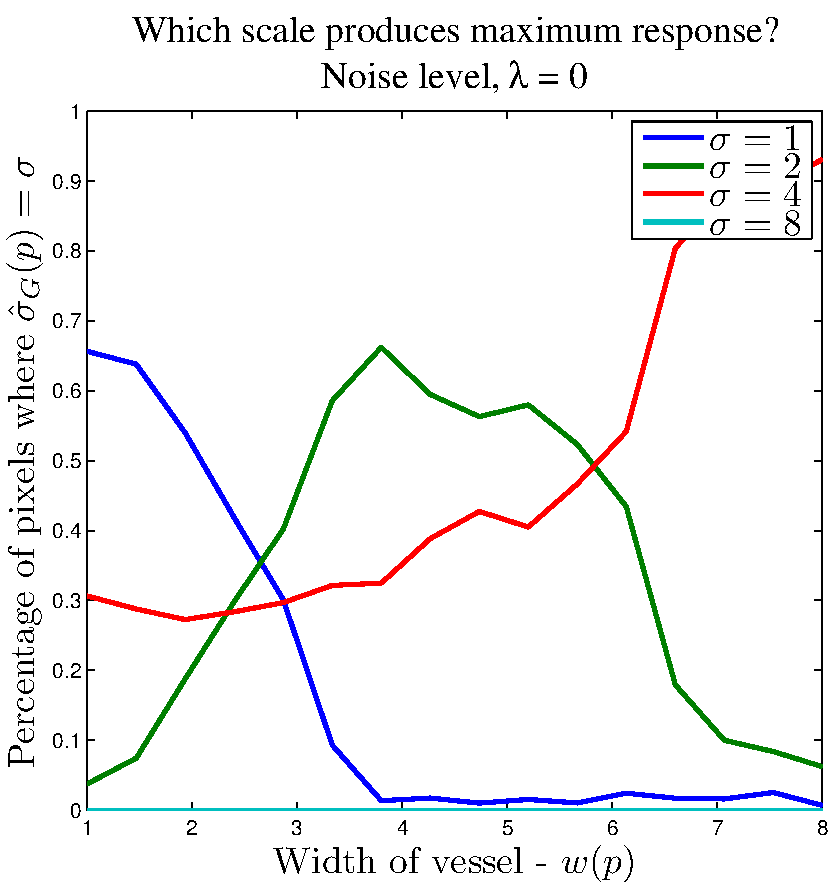
\includegraphics[width=0.18\textwidth]{figs/synthetic/syn_lines_g2d_scales_0} &
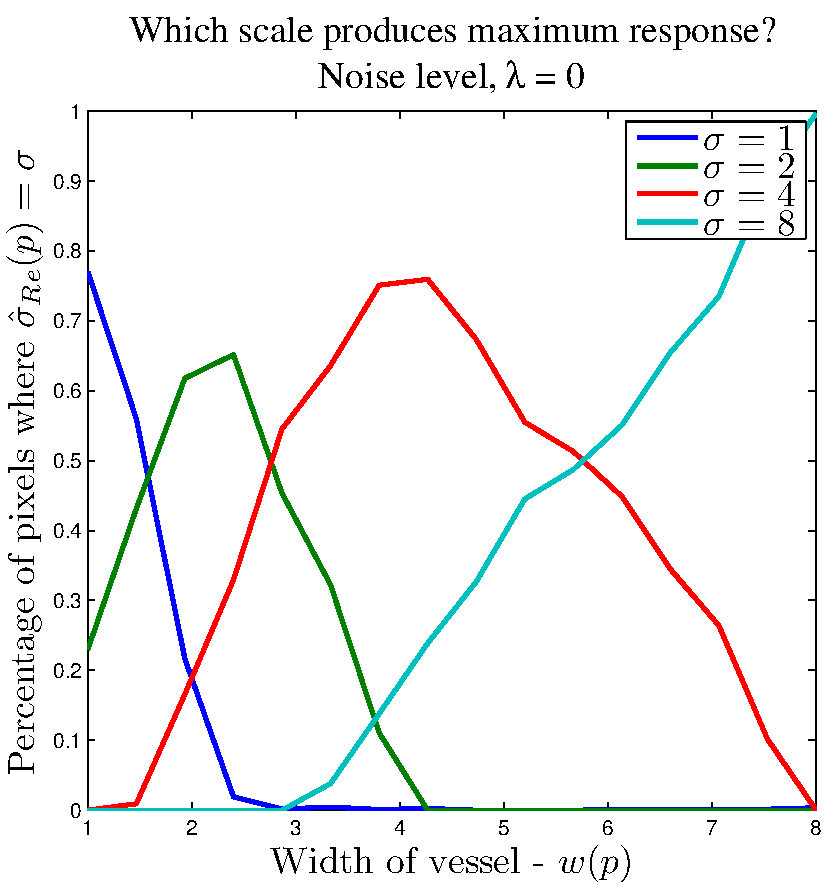
\includegraphics[width=0.18\textwidth]{figs/synthetic/syn_lines_gabor_scales_0} &
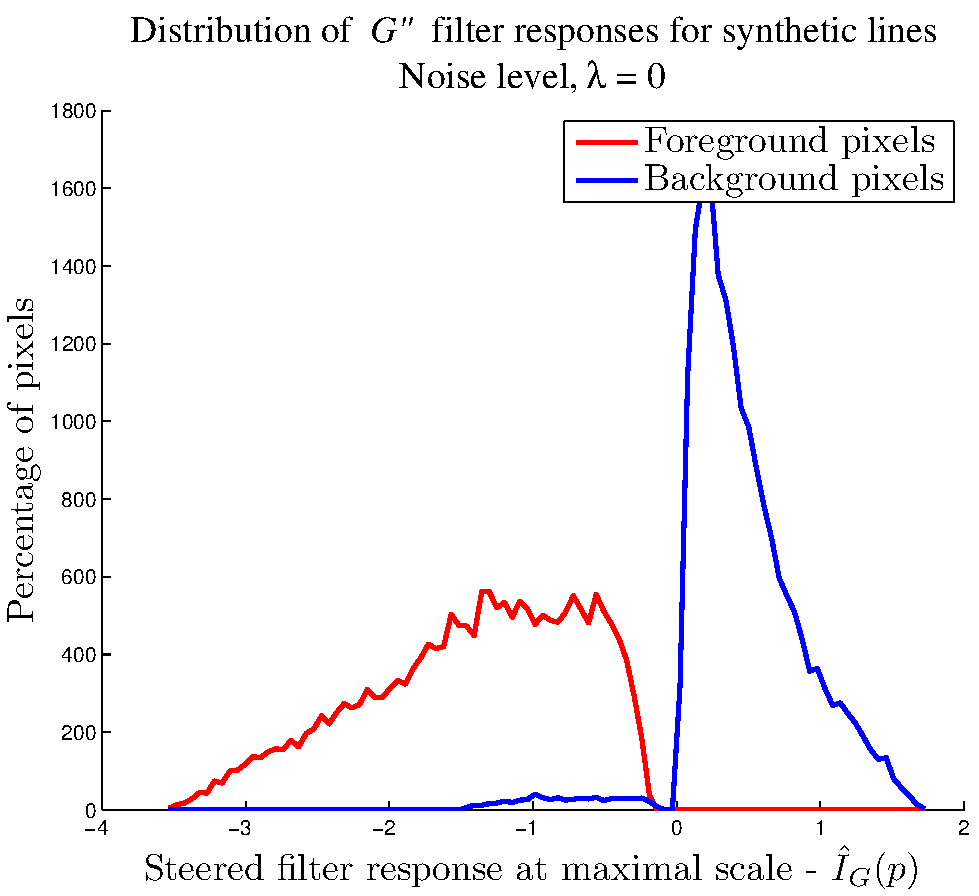
\includegraphics[width=0.18\textwidth]{figs/synthetic/syn_lines_g2d_responses_cdf_0} &
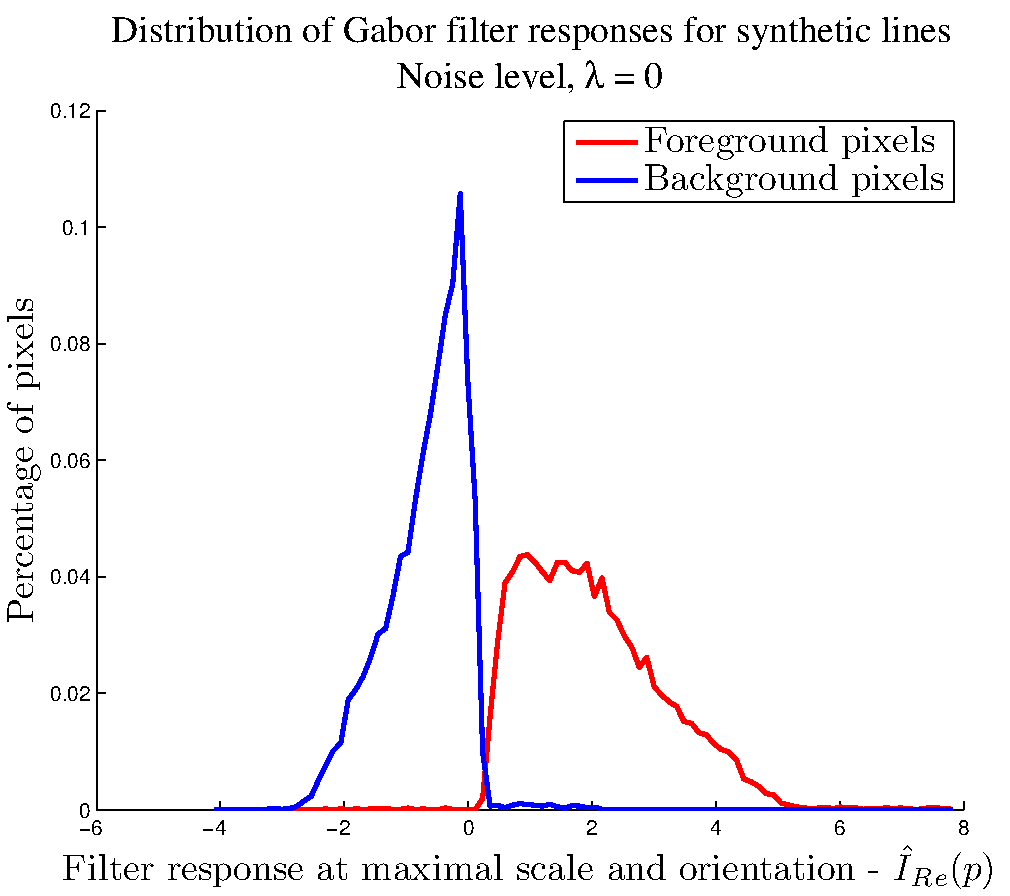
\includegraphics[width=0.18\textwidth]{figs/synthetic/syn_lines_gabor_responses_cdf_0} &
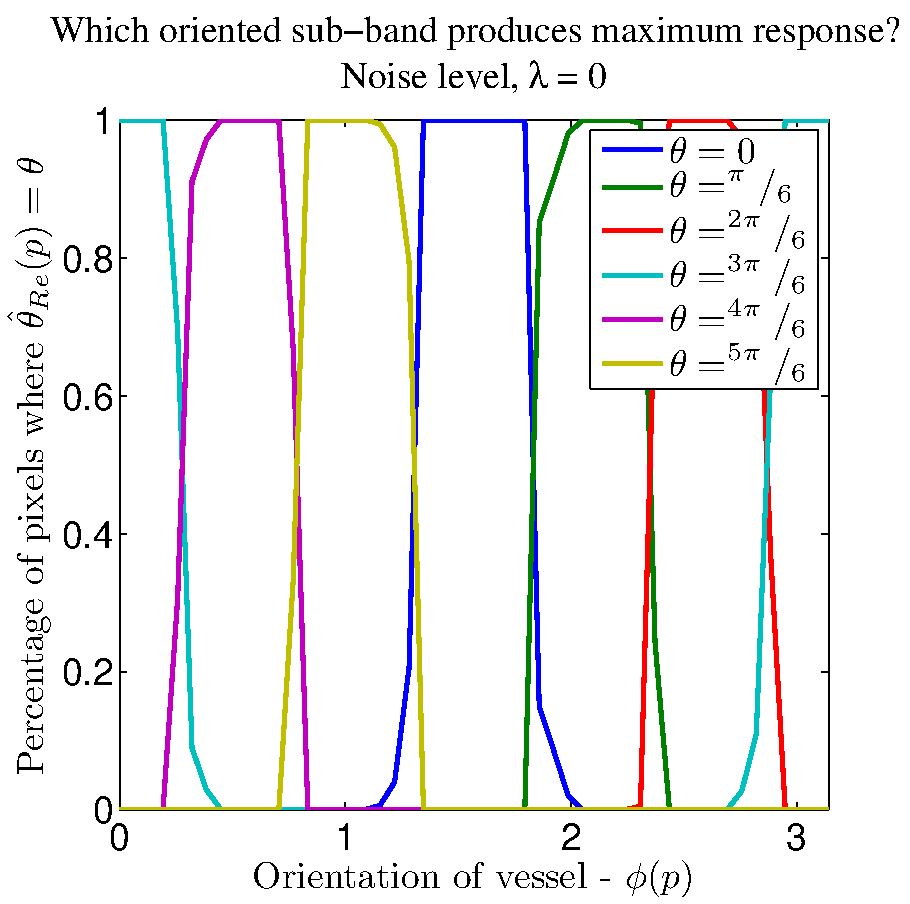
\includegraphics[width=0.18\textwidth]{figs/synthetic/syn_lines_gabor_ori_subbands_0} \\
%
$\eta=1$ &
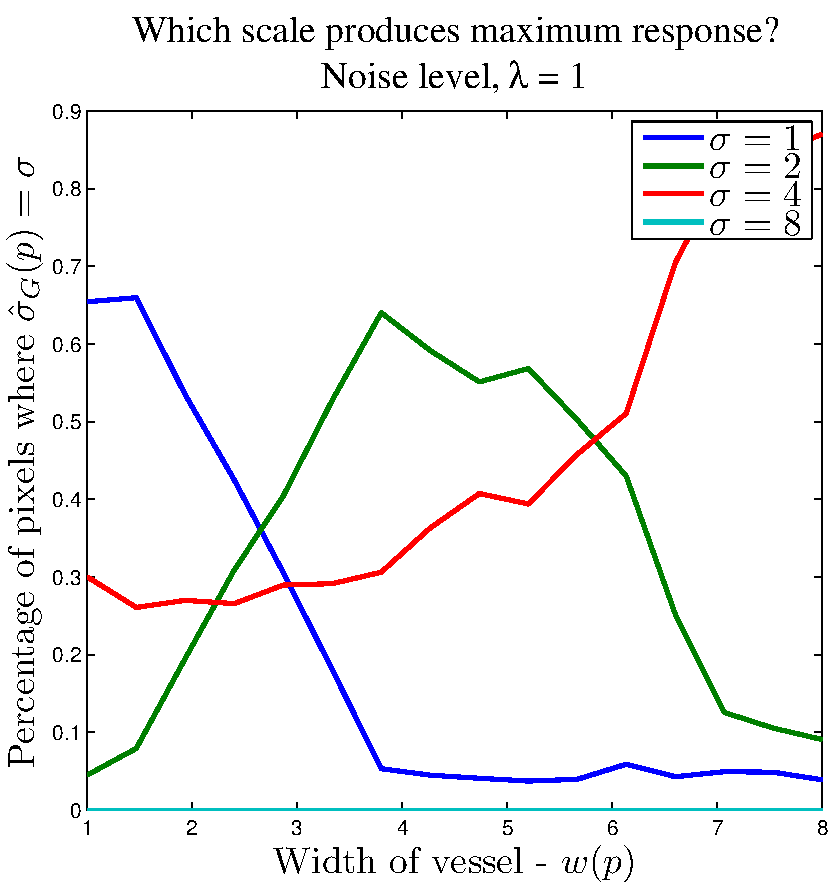
\includegraphics[width=0.18\textwidth]{figs/synthetic/syn_lines_g2d_scales_1} &
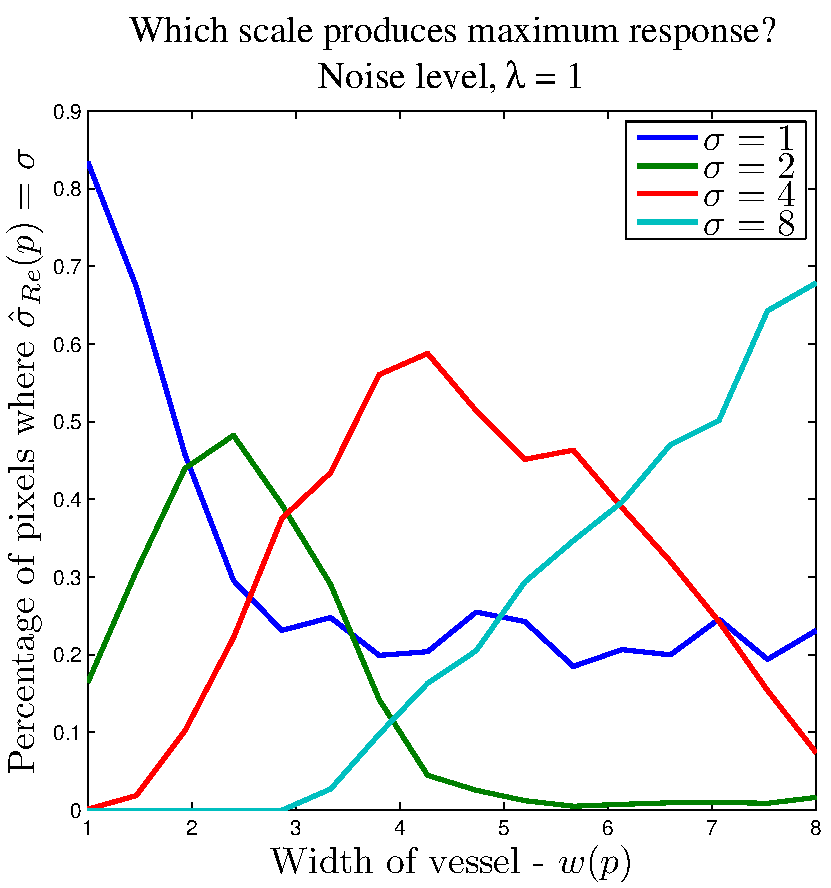
\includegraphics[width=0.18\textwidth]{figs/synthetic/syn_lines_gabor_scales_1} &
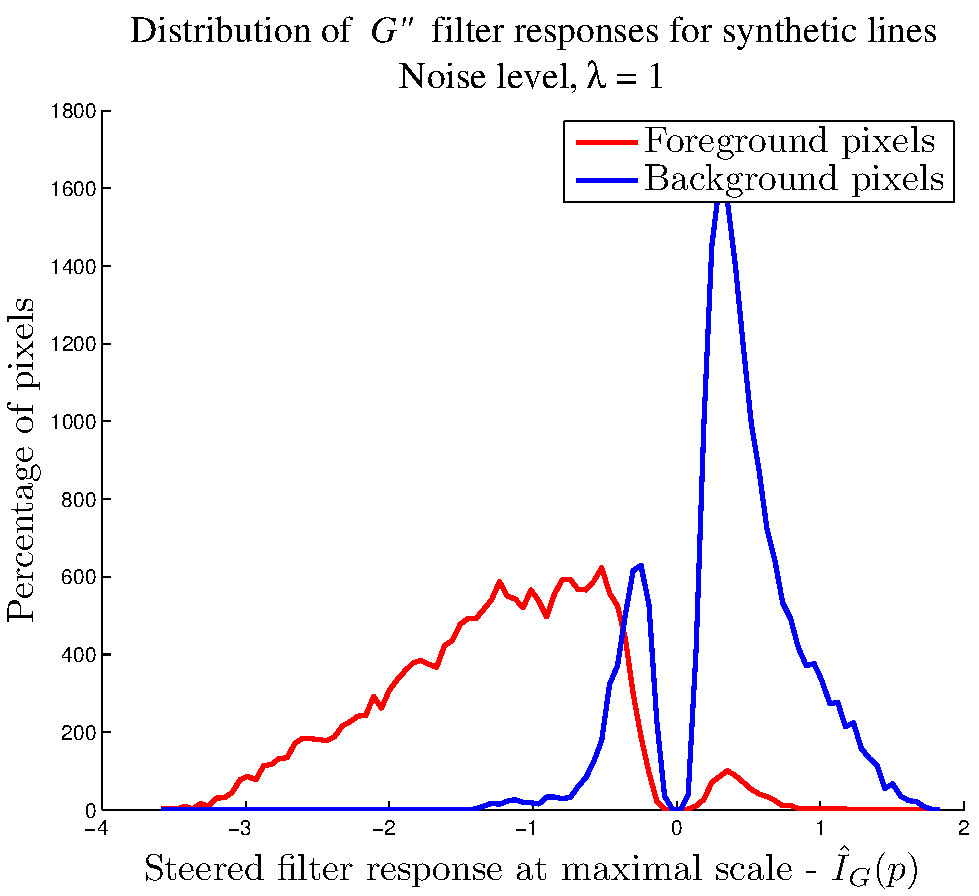
\includegraphics[width=0.18\textwidth]{figs/synthetic/syn_lines_g2d_responses_cdf_1} &
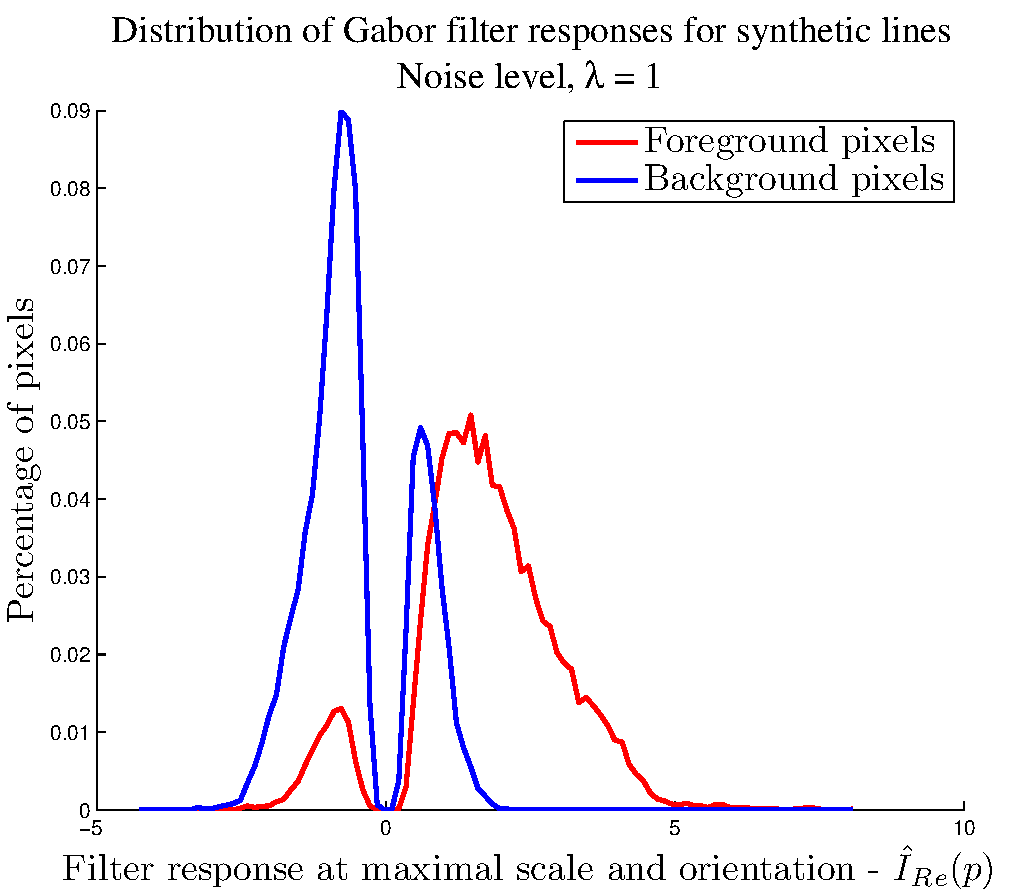
\includegraphics[width=0.18\textwidth]{figs/synthetic/syn_lines_gabor_responses_cdf_1} &
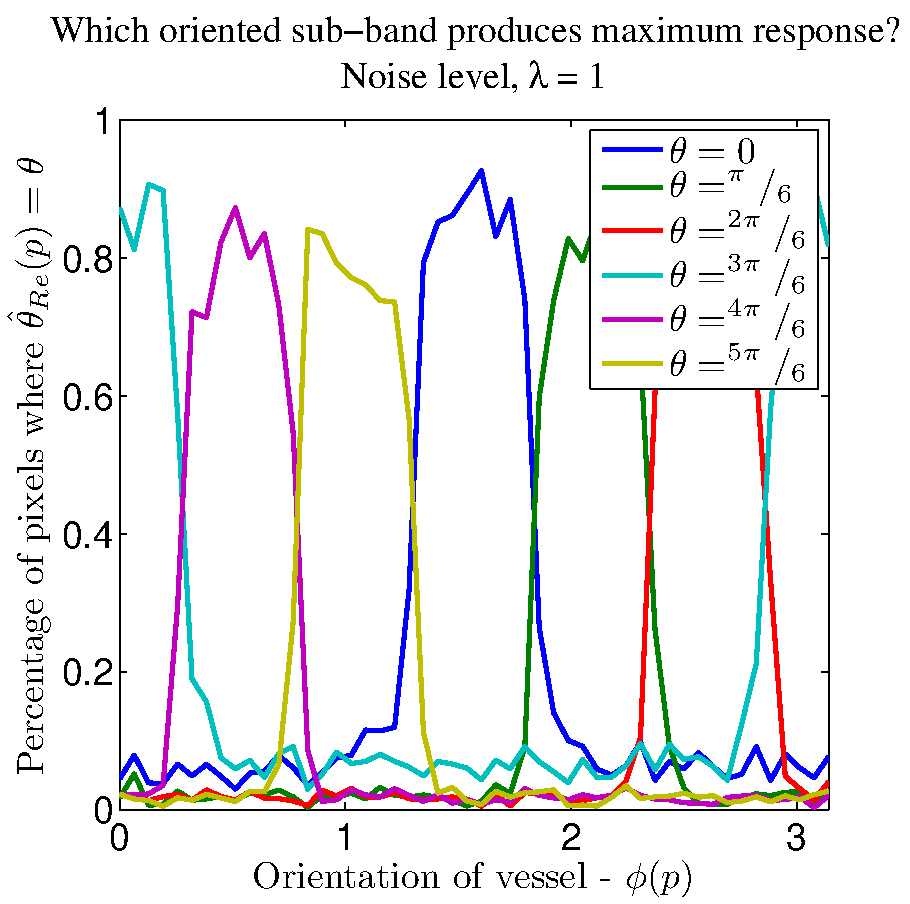
\includegraphics[width=0.18\textwidth]{figs/synthetic/syn_lines_gabor_ori_subbands_1} \\
%
$\eta=2$ &
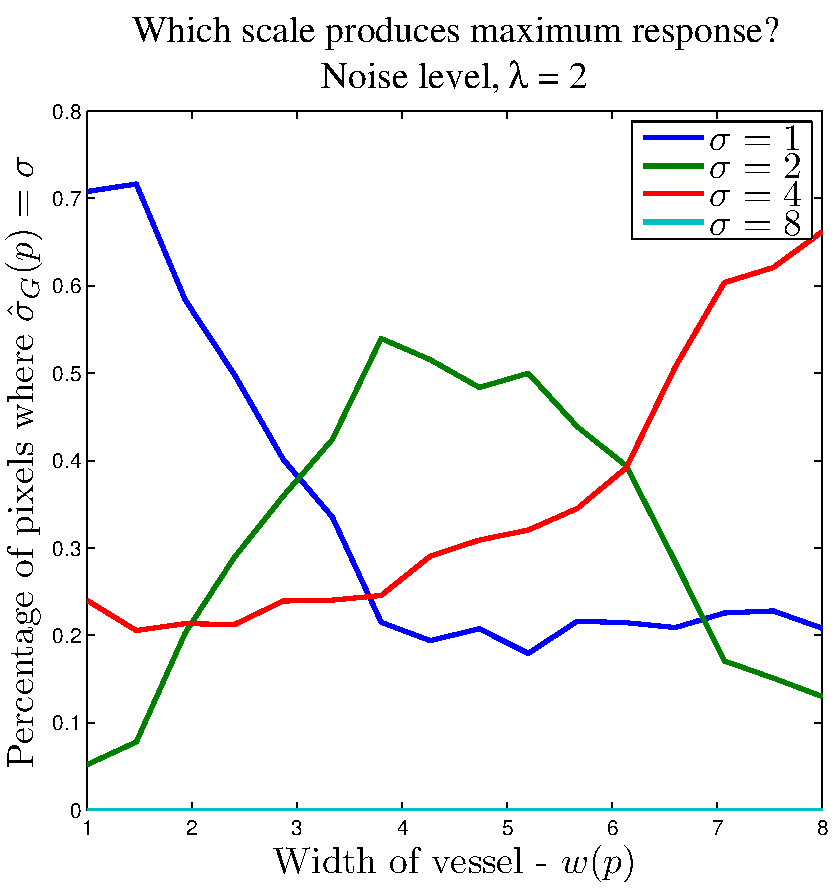
\includegraphics[width=0.18\textwidth]{figs/synthetic/syn_lines_g2d_scales_2} &
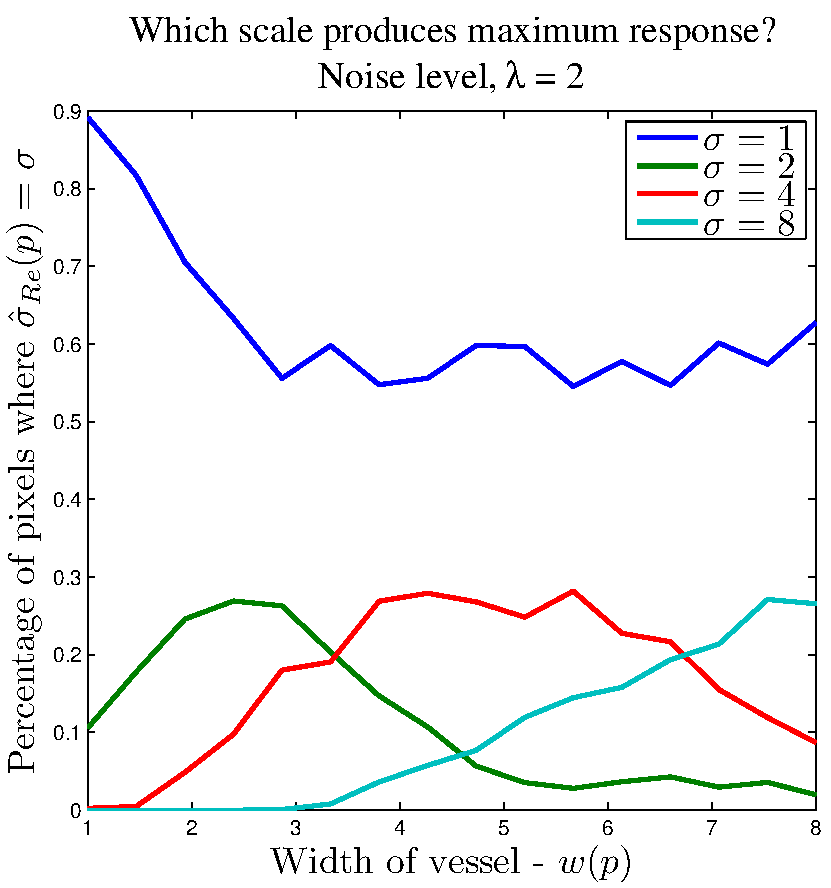
\includegraphics[width=0.18\textwidth]{figs/synthetic/syn_lines_gabor_scales_2} &
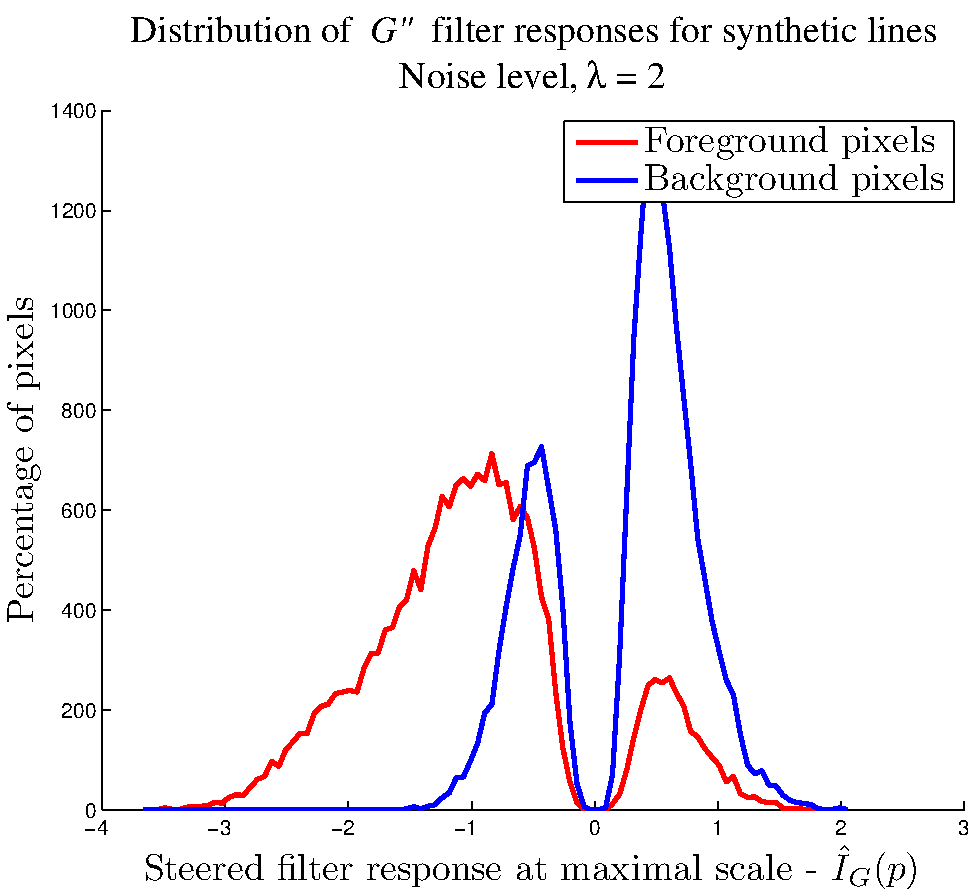
\includegraphics[width=0.18\textwidth]{figs/synthetic/syn_lines_g2d_responses_cdf_2} &
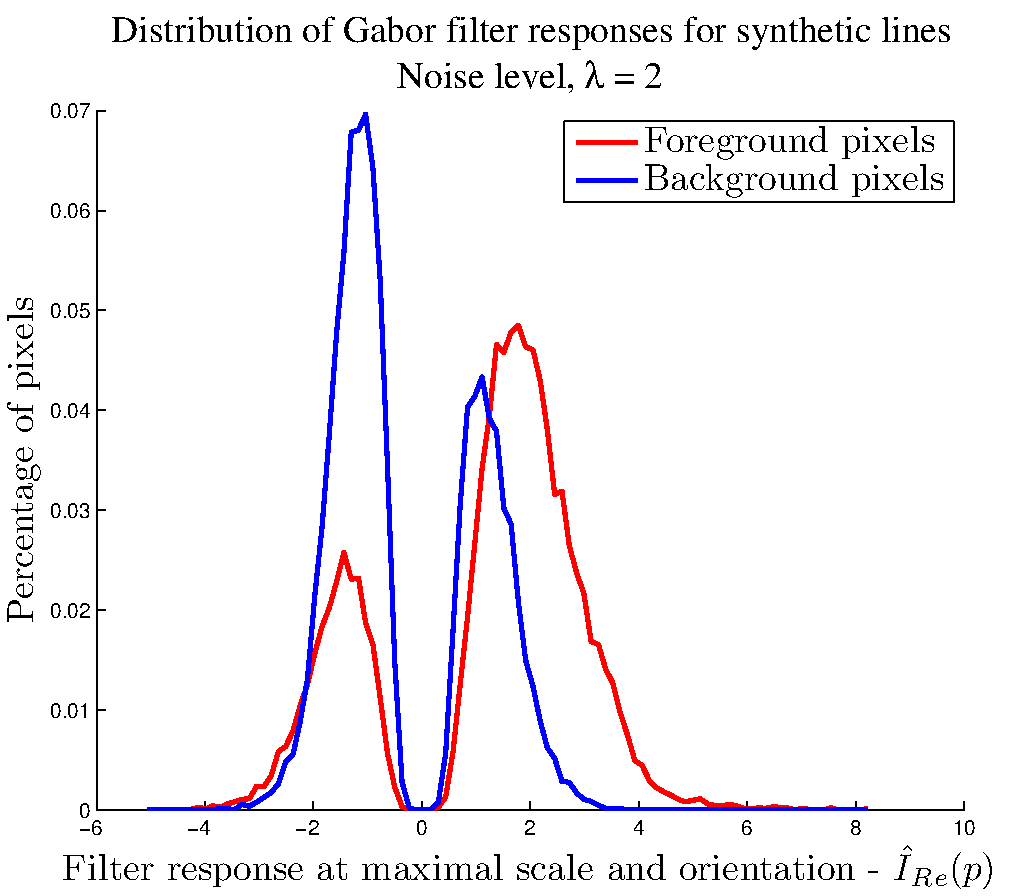
\includegraphics[width=0.18\textwidth]{figs/synthetic/syn_lines_gabor_responses_cdf_2} &
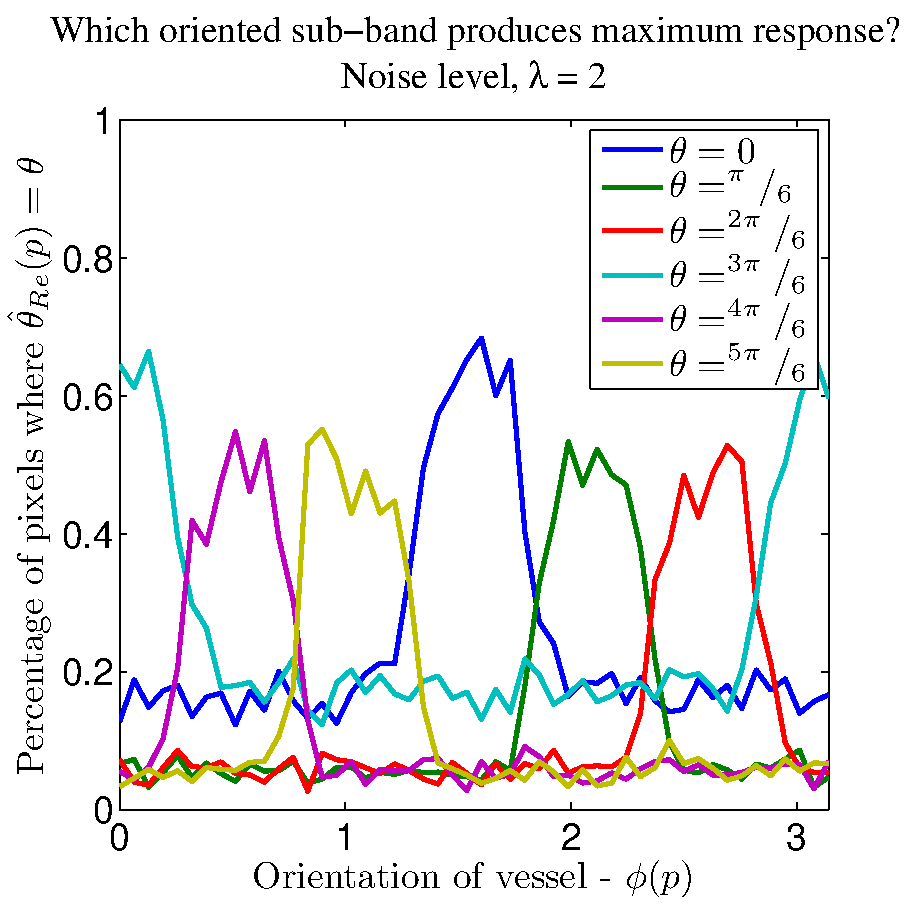
\includegraphics[width=0.18\textwidth]{figs/synthetic/syn_lines_gabor_ori_subbands_2} \\
%
$\eta=3$ &
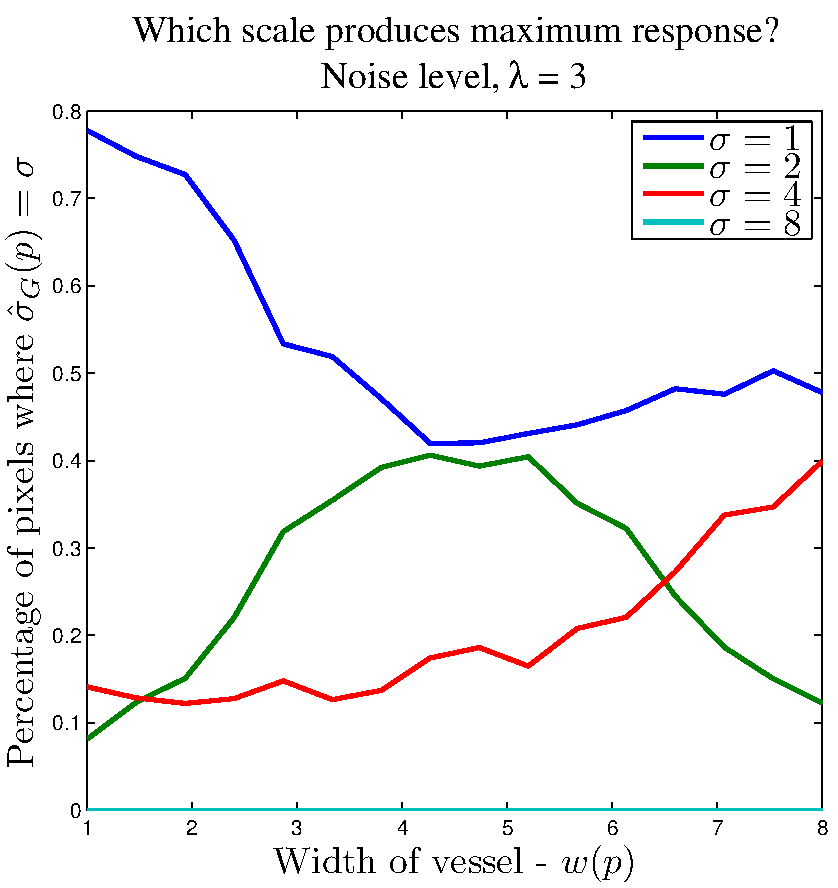
\includegraphics[width=0.18\textwidth]{figs/synthetic/syn_lines_g2d_scales_3} &
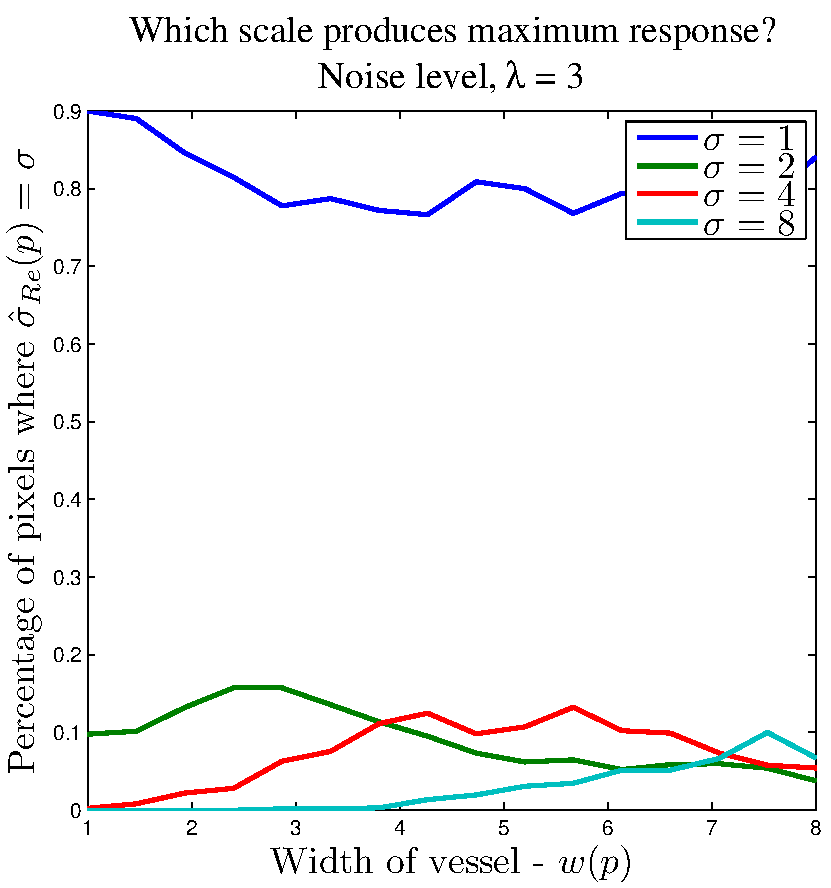
\includegraphics[width=0.18\textwidth]{figs/synthetic/syn_lines_gabor_scales_3} &
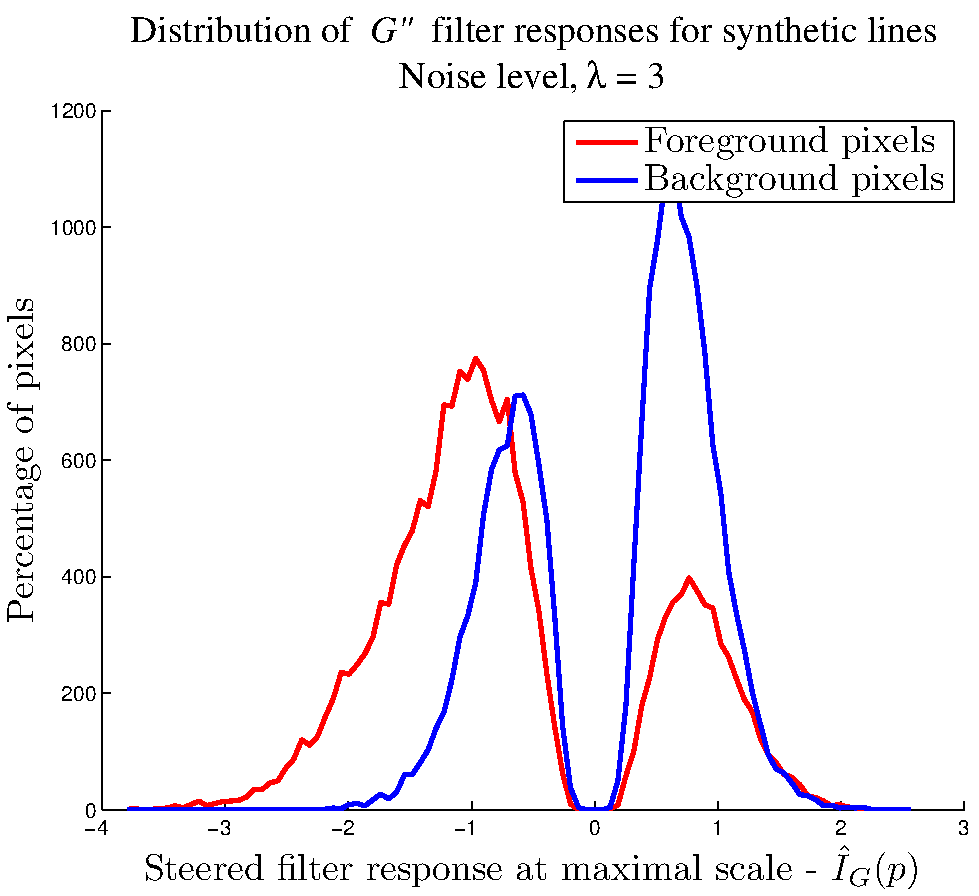
\includegraphics[width=0.18\textwidth]{figs/synthetic/syn_lines_g2d_responses_cdf_3} &
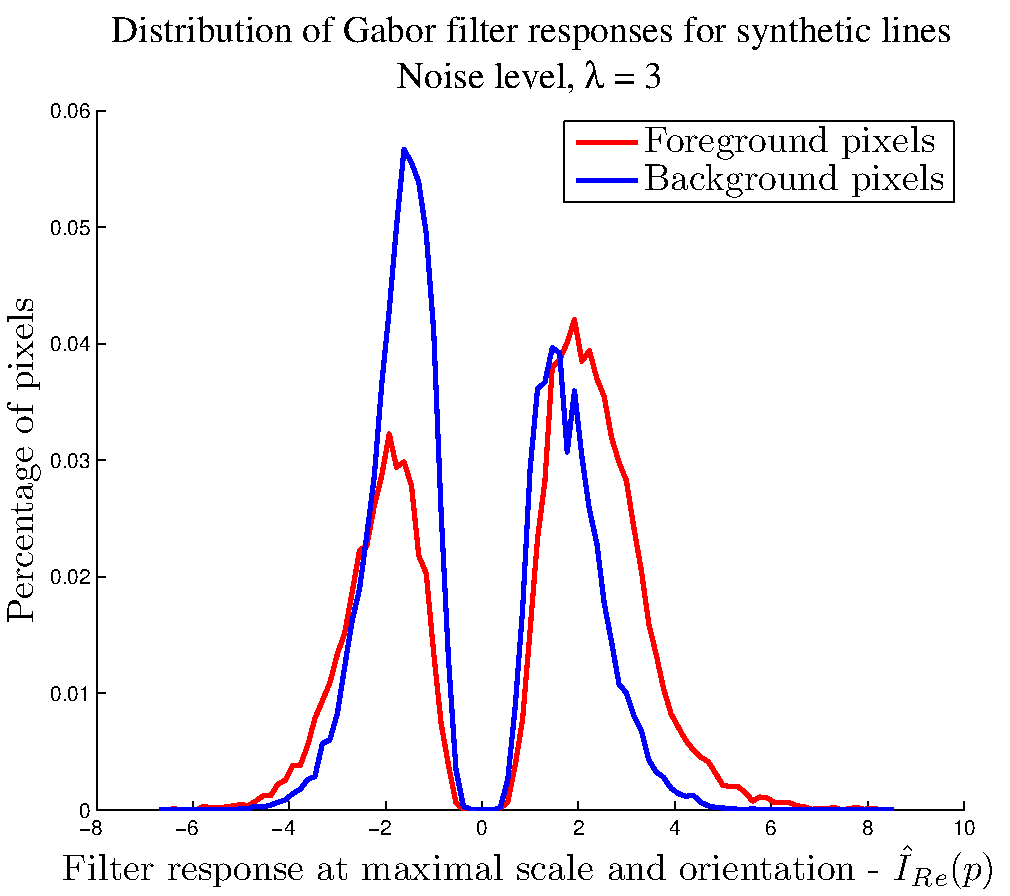
\includegraphics[width=0.18\textwidth]{figs/synthetic/syn_lines_gabor_responses_cdf_3} &
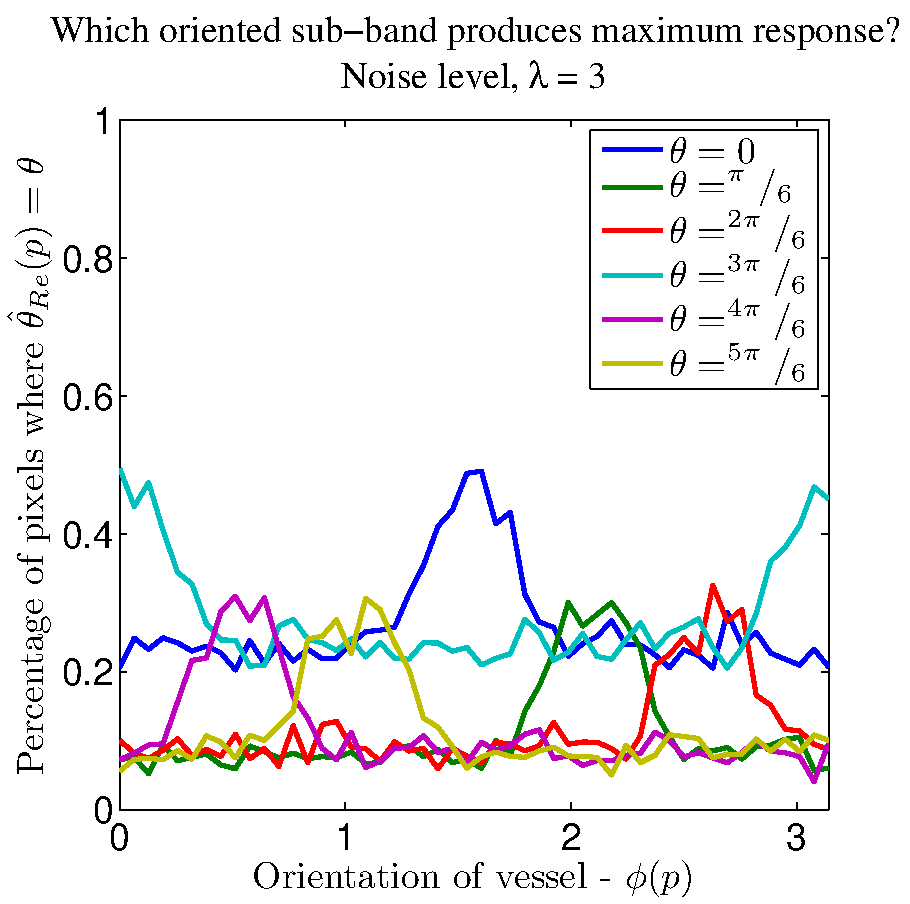
\includegraphics[width=0.18\textwidth]{figs/synthetic/syn_lines_gabor_ori_subbands_3} \\
 & (a) & (b) & (c) & (d) & (e)\\
\noalign{\smallskip}
\end{tabular}
}
%
\caption{Synthetic experiment results for (from top) noise levels $\eta=0,1,2,3$: Scale response as a function of CLS width to (a) Gaussian filters and (b) Gabor filters; CLS and background response distribution for (c) Gaussian filters and (d) Gabor filters; (e) Gabor filter response as a function of CLS orientation.}
\label{f:synthetic_exp1}
\end{figure*}


\begin{figure*}[t]
\centering
\resizebox{\textwidth}{!}{
\begin{tabular}{@{}l c c c c c@{}} % @{} removes padding around the edge of the table
%
$\eta=0$ &
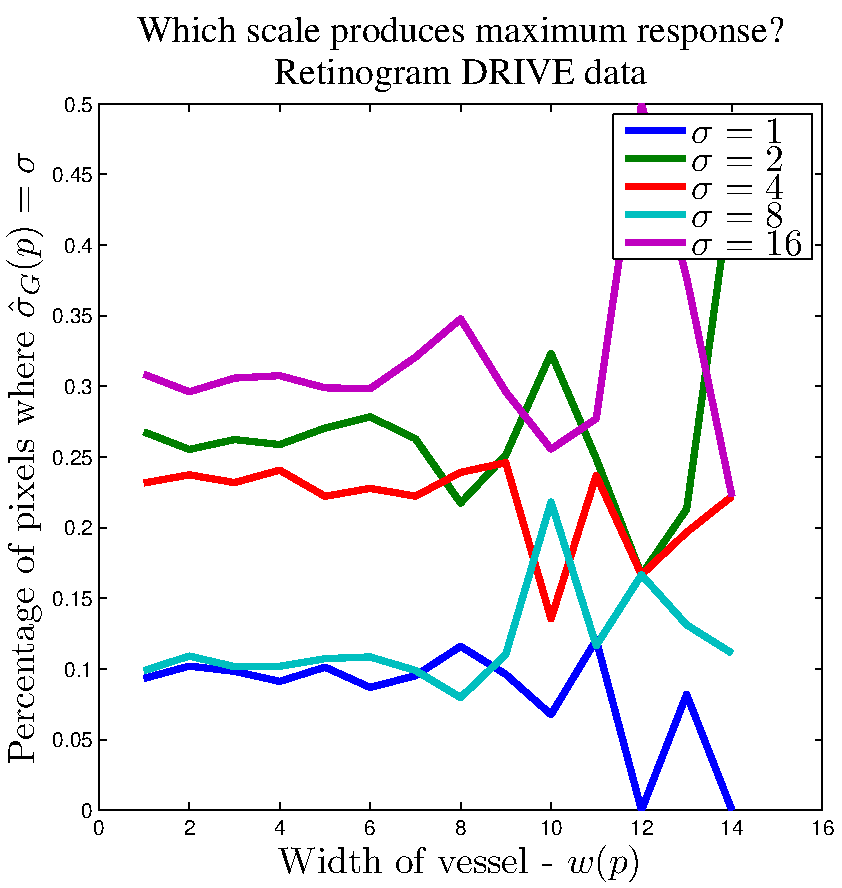
\includegraphics[width=0.18\textwidth]{figs/retina/ret_vessels_g2d_scales} &
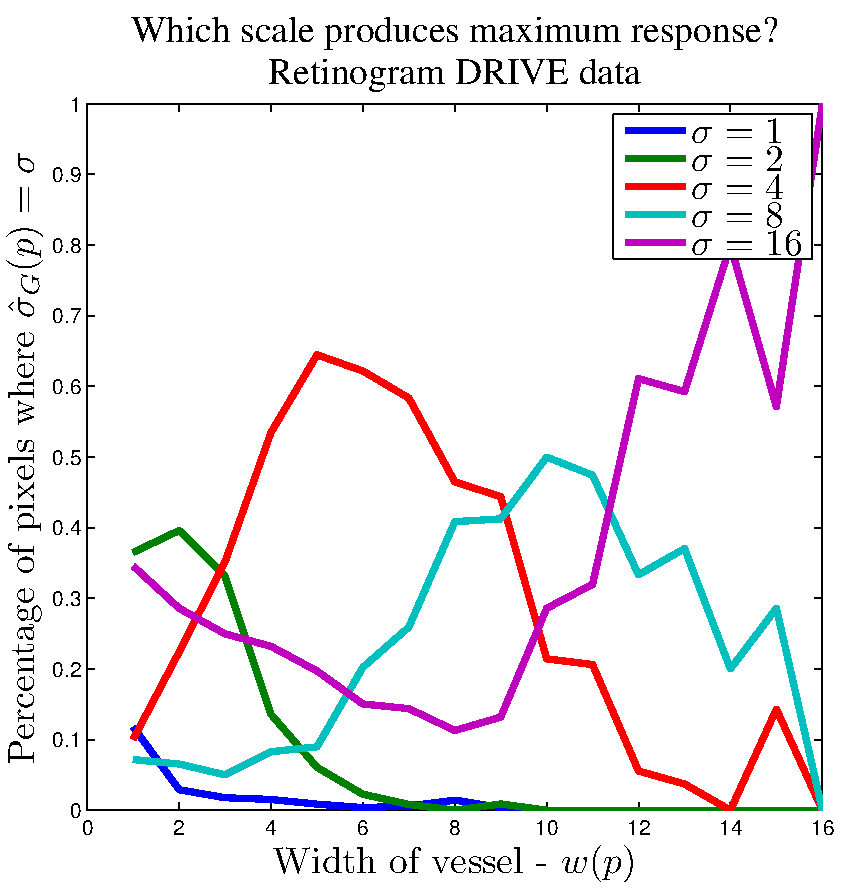
\includegraphics[width=0.18\textwidth]{figs/retina/ret_vessels_gabor_scales} &
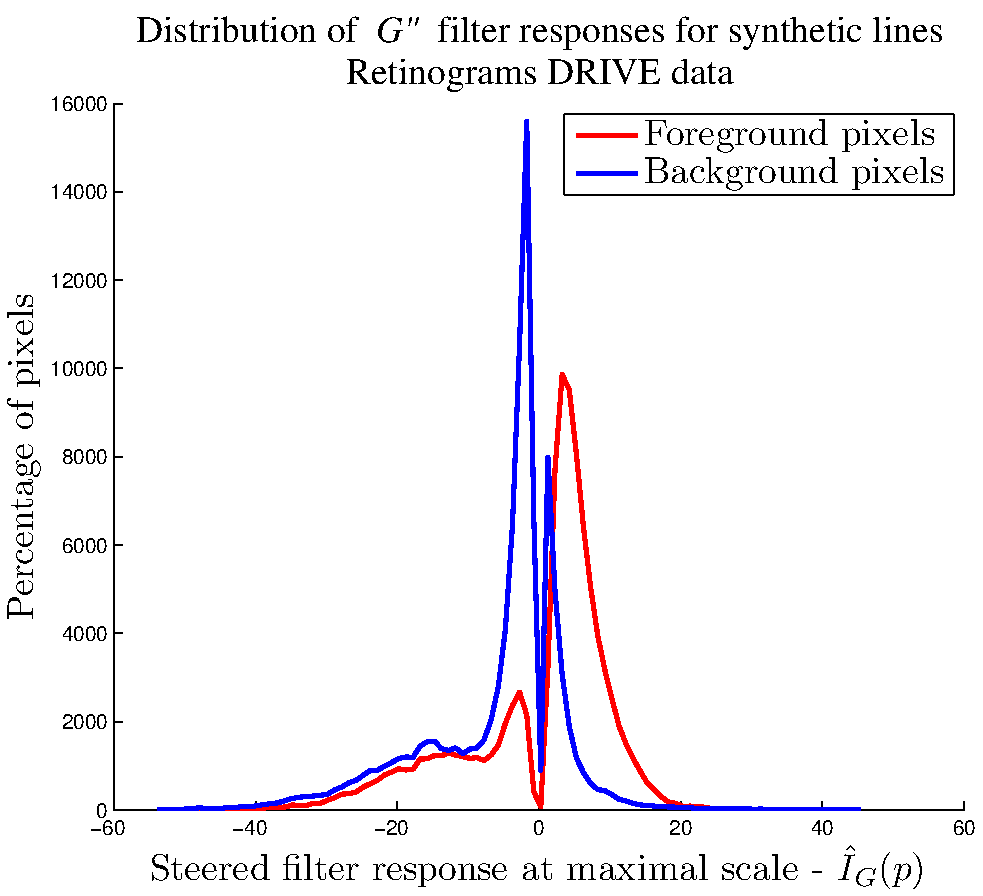
\includegraphics[width=0.18\textwidth]{figs/retina/ret_vessels_g2d_responses_cdf} &
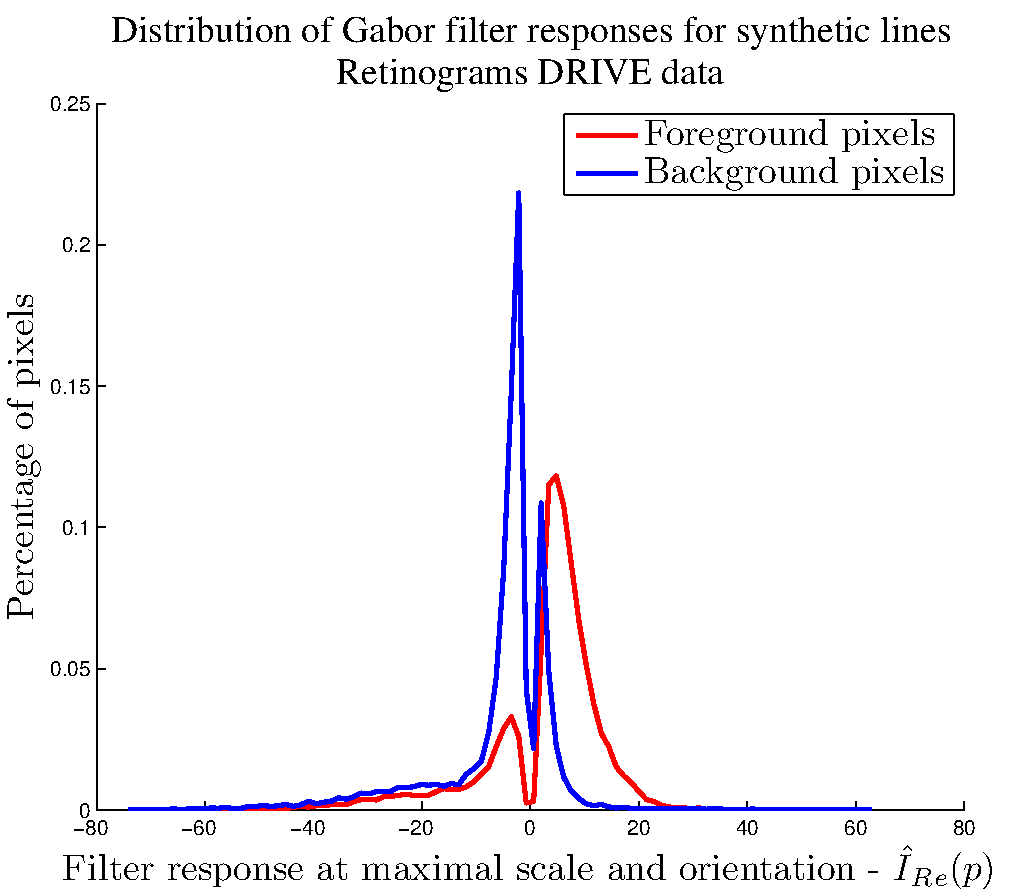
\includegraphics[width=0.18\textwidth]{figs/retina/ret_vessels_gabor_responses_cdf} &
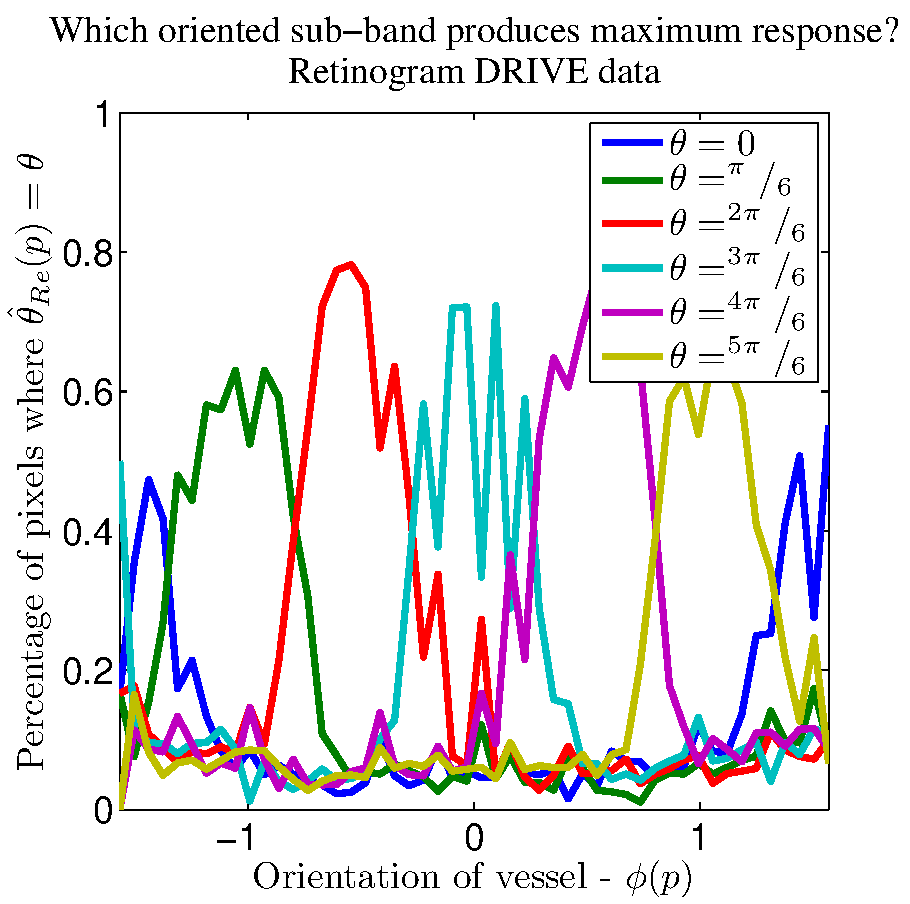
\includegraphics[width=0.18\textwidth]{figs/retina/ret_vessels_gabor_ori_subbands} \\
 & (a) & (b) & (c) & (d) & (e)\\
\noalign{\smallskip}
\end{tabular}
}
%
\caption{Experiment results for DRIVE dataset: Scale response as a function of CLS width to (a) Gaussian filters and (b) Gabor filters; CLS and background response distribution for (c) Gaussian filters and (d) Gabor filters; (e) Gabor filter response as a function of CLS orientation.}
\label{f:retina_exp1}
\end{figure*}
